\chapter{Interfejs użytkownika}
\label{cha:UI}
Niniejszy rozdział skupia się na szczegółowym opisie interfejsu użytkownika. Zostały przedstawione najważniejsze funkcję, które pomogą użytkownikom w korzystaniu z programu. Omówiono poszczególne warstwy wyświetlone na mapie, przełączanie między nimi oraz dodawanie nowych obiektów punktowych jak również dwuwymiarowych.
W pierwszej sekcji został przedstawiony widok główny aplikacji wraz z dokładnym omówieniem. W dalszej części tego rozdziału, zostały opisane kolejne warstwy. Na końcu przedstawiony został sposób, na dodawanie własnych obiektów.
\section{Widok główny aplikacji}
\label{sec:mainView}

Rys. \ref{mainView}. przedstawia widok główny aplikacji. W lewym górnym rogu znajdują się dwa przyciski: ''+'' oraz ''-''. Umożliwiają one przybliżanie i oddalanie widoku mapy. W prawym górnym rogu znajduję się menu wyboru wyświetlanej warstwy. Szczegóły dostępne w rozdziale \ref{sec:layerMenu}. Ponadto, użytkownik posiada możliwość, za pomocą myszki, przesuwania obecnie wyświetlanej mapy w dowolnym kierunku. Mapa pobierana jest w czasie rzeczywistym ze strony OpenStreetMap. Na dole znajdują się dwa nieaktywne pola typu input, służące do wyświetlania współrzędnych, jedna lista wyboru, przycisk do dodawania kolejnych współrzędnych oraz przycisk do dodawania obiektu. Lista wyboru umożliwia wybranie jednej z sześciu kategorii:
\begin{itemize}
\item \textbf{traffic signal} - sygnalizacji świetlnej
\item \textbf{pedestrian crossing} - przejście dla pieszych
\item \textbf{rail crossing} - przejazd kolejowy
\item \textbf{bus stop} - przystanek autobusowy lub tramwajowy
\item \textbf{schools} - szkoła
\item \textbf{shops churches} - sklep lub miejsce kultu religijnego
\end{itemize}

\newpage
\begin{figure}[h]
\caption{Widok główny aplikacji}
\label{mainView}
\centering
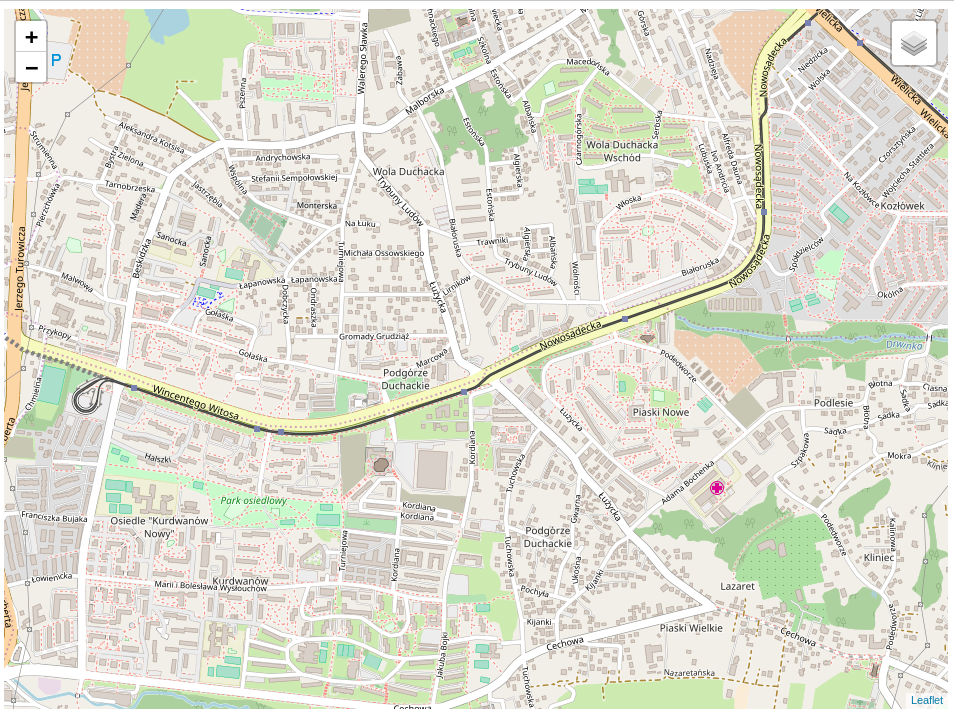
\includegraphics[width=1.02\textwidth]{mainScreen}
\end{figure}

\newpage

\section{Menu wyboru warstw}
\label{sec:layerMenu}

Rys. \ref{sec:mainLayerView}. przedstawia menu wyboru warstw. Dostępny jest dopiero po najechaniu kursorem myszy w prawy górny róg. Umożliwia wyświetlanie na mapie elementów, które użytkownik w danej chwili potrzebuje. 

\begin{figure}[h]
\caption{Menu wyboru warstw}
\label{sec:mainLayerView}
\centering
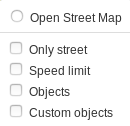
\includegraphics[width=0.55\textwidth]{layerMenu}
\end{figure}

Menu wyboru warstw, Rys. \ref{sec:mainLayerView}, składa się z 35 elementów:
\begin{itemize}
\item \textbf{Only street} - służy do zaznaczania na mapie, wszystkich dostępnych ulic. Więcej szczegółów znajduje się w rozdziale \ref{sec:onlyStreet}
\item \textbf{One way streets} - zaznacza na mapie drogi jednokierunkowe
\item \textbf{pedestrian crossing, pedestrian crossing street i pedestrian crossing speed} - zaznacza na mapie odpowiednio przejścia dla pieszych, ulice na których się one znajdują oraz ograniczenia prędkości. Szczegóły zostały opisane w rozdziale \ref{sec:pedestrialCrossing} 
\item \textbf{rail crossing, rail crossing street i rail crossing speed} - zaznacza na mapie odpowiednio przejazdy kolejowe, ulice na których się one znajdują oraz ograniczenia prędkości. Szczegóły zostały opisane w rozdziale \ref{sec:railCrossingMain} 
\item \textbf{traffic signal, traffic signal street i traffic signal speed} - zaznacza na mapie odpowiednio sygnalizację świetlną, ulice na których się one znajdują oraz ograniczenia prędkości. Szczegóły zostały opisane w rozdziale \ref{sec:trafficSignalMain} 
\item \textbf{bus stop, bus stop bounding box, bus stop street, bus stop start oraz bus stop end} - zaznacza na mapie odpowiednio przystanki autobusowe i tramwajowe, minimalny obszar pokrywający te przystanki powiększony o 5 metrów, ulice na których znajdują się przystanki, znaki początku oraz końca ograniczenia prędkości. Szczegóły opisane zostały w rozdziale \ref{sec:busStopsMain}
\item \textbf{school, school bounding box, school street, school start oraz school end} - zaznacza na mapie odpowiednio szkoły, minimalny obszar pokrywający szkoły powiększony o 30 metrów, ulice przy których znajdują się szkoły, znaki początku oraz końca ograniczenia prędkości. Szczegóły opisane zostały w rozdziale \ref{sec:schoolsMain}
\item \textbf{shops churches, shops churches bounding box, shops churches street, shops churches start oraz shops churches end} - zaznacza na mapie odpowiednio sklepy i miejsca kultów religijnych, minimalny obszar pokrywający te obiekty powiększony o 30 metrów, ulice przy których znajdują się te obiekty, znaki początku oraz końca ograniczenia prędkości. Szczegóły opisane zostały w rozdziale \ref{sec:shoopsChurchesMain}
\item \textbf{number of lanes, number of lanes speed} - zaznacza na mapie odpowiednio liczbę pasów ruchu oraz prędkość z nimi związaną. Szczegóły zostały opisane w rozdziale \ref{sec:laneNumber}
\item \textbf{type of road speed} - zaznacza na mapie ograniczenia prędkości związane z typem nawierzchni. Szczegóły zostały opisane w rozdziale \ref{sec:typeOfRoad}
\item \textbf{Curves, Curves speed start, Curves speed end} - zaznacza na mapie odpowiednio zakręty, znaki początku i końca ograniczenia prędkości dotyczące zakrętów. Szczegóły zostały opisane w rozdziale \ref{sec:zakretyMain}
\item \textbf{finished speed, finished speed street} - Najważniejsza warstwa. Umieszcza ograniczenia prędkości na mapie, wyznaczone na podstawie wszystkich powyższych składowych. Szczegóły zostały opisane w rozdziale \ref{sec:speedLimitLocalization}
\end{itemize}

Istotną funkcjonalnością jest możliwość wyświetlania dowolnych kombinacji warstw. Użytkownik może zaznaczyć dowolną liczbę widoków, które zostaną wyświetlone na głównej mapie.

\newpage
\section{Widok zaznaczonych ulic}
\label{sec:onlyStreet}

Rys. \ref{sec:onlyStreetMap} przedstawia mapę, na której zaznaczone są poszczególne odcinki dróg. Reprezentowane są przez niebieskie linie łamane, przebiegającą przez sam jej środek. Zostały uwzględnione różnego rodzaju klasy dróg, takie jak: 
\begin{itemize}
\item autostrady
\item drogi ekspresowe
\item drogi główne ruchu przyspieszonego
\item drogi główne
\item drogi zbiorcze
\item drogi lokalne
\item drogi dojazdowe
\end{itemize}

\begin{figure}[h]
\caption{Widok zaznaczonych ulic}
\label{sec:onlyStreetMap}
\centering
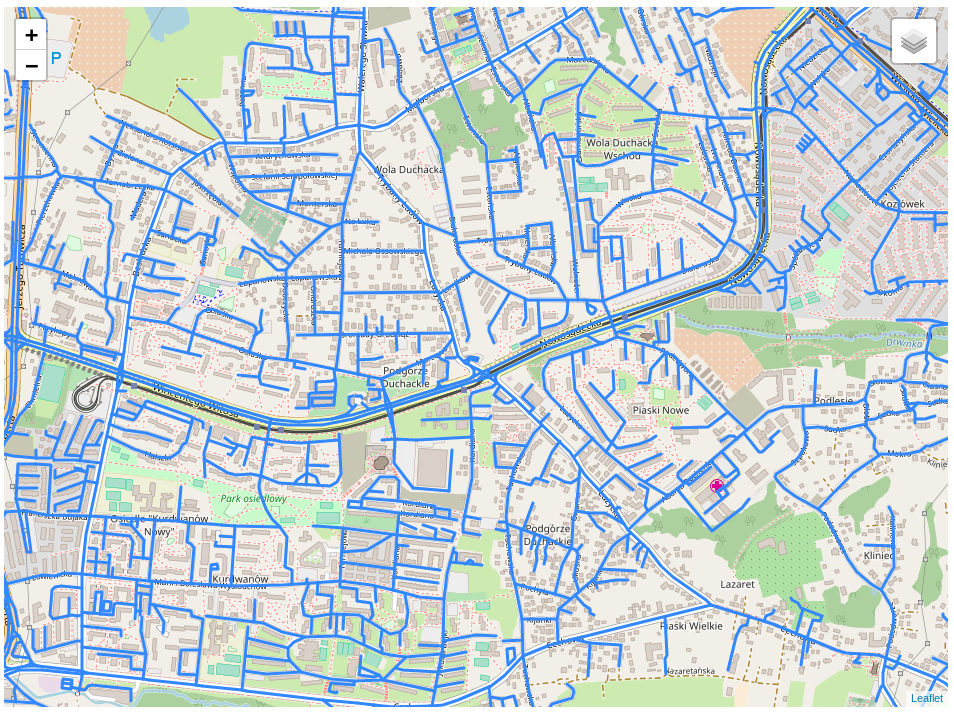
\includegraphics[width=1.03\textwidth]{onlyStreet}
\end{figure}

\newpage
\section{Dodawanie własnych obiektów}
\label{sec:addedCustomObjects}

Jednym z kluczowych elementów działania aplikacji jest dodawanie własnych obiektów. Użytkownik ma możliwość dodać zarówno obiekty dwuwymiarowowe jak i reprezentowane przez pojedynczy punkt. Rys. \ref{sec:addObject} przedstawia widok dodawania nowego obiektu

\begin{figure}[h]
\caption{Widok dodawania obiektów}
\label{sec:addObject}
\centering
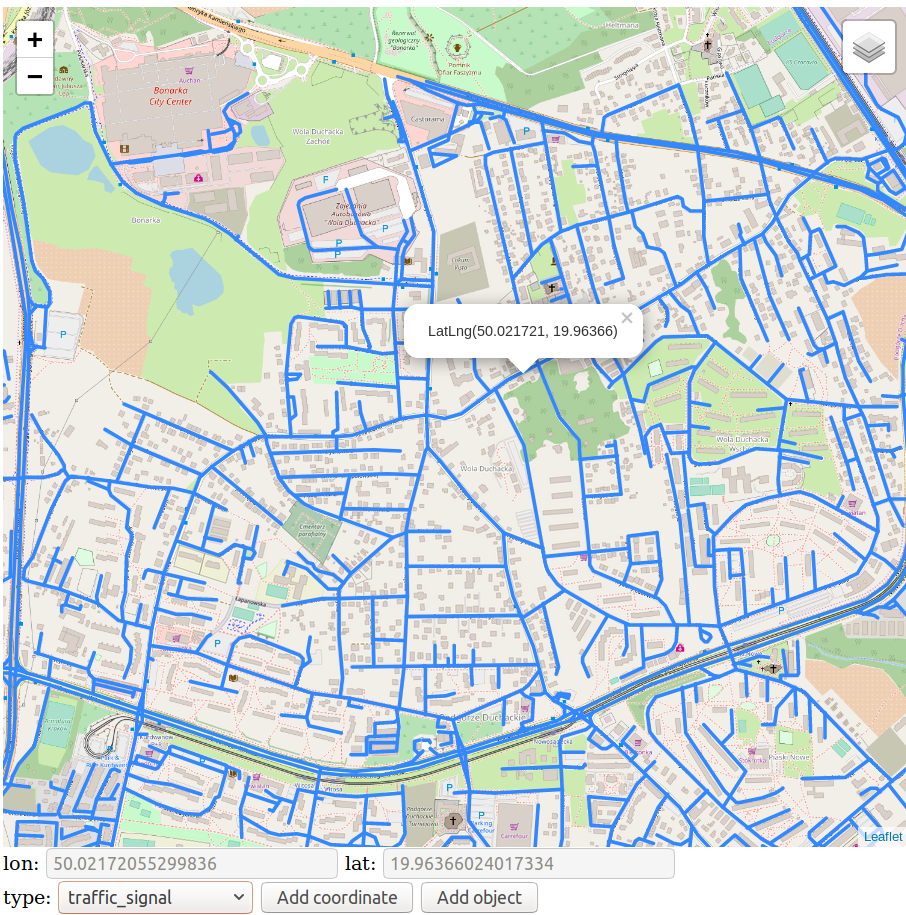
\includegraphics[width=1.07\textwidth]{addObject}
\end{figure}

\newpage
\subsection{Dodawanie obiektów reprezentowanych przez pojedynczy punkt}
Do obiektów reprezentowanych przez pojedynczy punkt zaliczyć można:
\begin{itemize}
\item Przejścia dla pieszych
\item Sygnalizacje świetlne
\item Przejazdy kolejowe
\end{itemize}

Algorytm dodawania obiektów wygląda następująco:
\begin{enumerate}
\item Kliknąć na mapie w dowolnie wybrany punkt - pojawi się dymek z widocznymi współrzędnymi, oraz zostaną wypełnione dwa pola pod mapą - widoczne na rysunku: \ref{sec:addObject}
\item Wybrać z listy rozwijanej jeden z trzech typów: przejście dla pieszych, sygnalizację świetlną lub przejazd kolejowy
\item Nacisnąć przycisk: Add object - obiekt został dodany do mapy.
\end{enumerate} 

\subsection{Dodawanie obiektów reprezentowanych przez zbiór punktów}
Do obiektów reprezentowanych przez zbiór punktów zaliczyć można:
\begin{itemize}
\item Przystanki autobusowe i tramwajowe
\item Szkoły
\item Place zabaw
\item Sklepy
\item Obiekty kultów religijnych
\end{itemize}

Algorytm dodawania obiektów wygląda następująco:
\begin{enumerate}
\item Kliknąć na mapie w dowolnie wybrany punkt będącym jednym z rogów nowo dodawanego obiektu dwuwymiarowego - pojawi się dymek z widocznymi współrzędnymi, oraz zostaną wypełnione dwa pola pod mapą - widoczne na rysunku: \ref{sec:addObject}
\item Nacisnąć przycisk: Add coordinates - współrzędne wybranego punktu zostały zapisane w pamięci
\item Powtarzać krok 1 i 2, do momentu aż cały obiekt nie zostanie oznaczony
\item Wybrać z listy rozwijanej jeden z trzech typów: przystanek autobusowy lub tramwajowy, szkoła, plac zabaw, sklep lub obiekt kultu religijnego
\item Nacisnąć przycisk: Add object - obiekt został dodany do mapy.
\end{enumerate} 